En optimisant également le nombre d'ouvriers, nous obtenons un graphe qui suit beaucoup mieux la courbe de demande: l'usine tourne toujours au maximum, mais en adaptant son nombre d'ouvriers. Il y a moins de stock, largement moins d'heures supplémentaires, et la sous-traitance a même totalement disparu.

Cependant, puisque l'on n'a pas imposé l'intégralité des variables, nous obtenons un nombre d'ouvriers non-entier, ce qui n'est pas possible en réalité.

\begin{figure}[H]
    \centering
    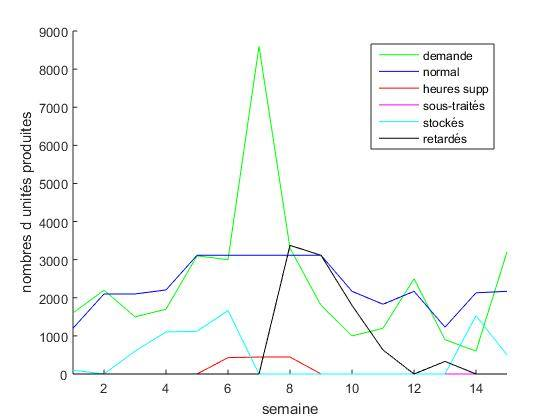
\includegraphics[width=0.8\textwidth]{graphes/q8_01.jpg}
    \caption{Graphe de la production à personnel variable non-entier}
    \label{fig:q8_01}
\end{figure}

\begin{figure}[H]
    \centering
    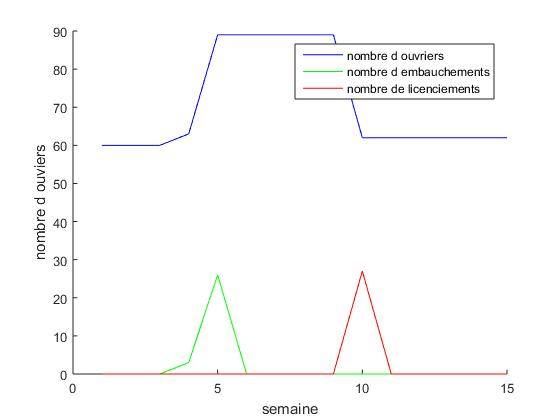
\includegraphics[width=0.8\textwidth]{graphes/q8_02.jpg}
    \caption{Graphe de la variation du personnel non-entier}
    \label{fig:q8_02}
\end{figure}
